\documentclass[A4,12PT, english, twocolumn]{journal}
\usepackage{amsmath,amssymb,amsfonts}
\usepackage[margin=0.7in]{geometry}
\usepackage{graphicx}
\usepackage{enumitem}
\usepackage{xcolor}
\usepackage{hyperref}
\usepackage{tabularray}
\usepackage{multicol}
\usepackage{tikz}
\usepackage{circuitikz}
\usepackage{scalerel}
\usepackage{pict2e}
\usepackage{tkz-euclide}
\usetikzlibrary{calc}
\usetikzlibrary{patterns,arrows.meta}
\usetikzlibrary{shadows}
\usetikzlibrary{external}

%pgfplots
\usepackage{pgfplots}
\pgfplotsset{compat=newest}
\usepgfplotslibrary{statistics}
\usepgfplotslibrary{fillbetween}

\def\infinity{\rotatebox{90}{8}}

% Hiperlink
\hypersetup{
    colorlinks=true,
    linkcolor=blue,
    filecolor=magenta,      
    urlcolor=cyan,
    pdftitle={Overleaf Example},
    pdfpagemode=FullScreen,
}
%\usepackage{style}
\NewDocumentCommand{\Log}{o}{%
\IfNoValueTF{#1}{}{{}^{#1}\!}\log}%
  
%command buat logaritma dengan basisnya di pojok kiri
%\textheight=17cm
%\textwidth=10cm
%\usepackage{blindtext}
\setenumerate[1]{itemsep=0,5cm}
\setenumerate[2]{topsep=5pt, itemsep=5pt, label=\textbf{\Alph*}.}

\title{Matematika Saintek \& Fisika UTUL UGM 2016 Kode 381}
\author{Fauzan Akbar Sukandar Putra \\ \LaTeX}

\begin{document}

\maketitle

%\begin{minipage}{0.5\textwidth}
\begin{enumerate}


%1%
\item Persamaan lingkaran yang berpusat di titik $(-1,2)$ dan menyinggung garis $2y+3x-14=0$ adalah\dots
    \begin{enumerate}
        \item $(x-1)^2+(y+2)^2=10$
        \item $(x+1)^2+(y-2)^2=10$
        \item $(x-1)^2+(y+2)^2=13$
        \item $(x+1)^2+(y-2)^2=13$
        \item $(x+1)^2+(y-2)^2=15$
    \end{enumerate}

%2%
\item Jika $\frac{1-\sec{x}}{\tan{x}}=5$, maka $\frac{1+\sec{x}}{\tan{x}}=$ adalah\dots
    \begin{enumerate}
        \item $5$
        \item $\frac{1}{5}$
        \item $\frac{1}{25}$
        \item $-\frac{1}{5}$
        \item $-5$
    \end{enumerate}

%3%
\item Diketahui $\theta$ merupakan sudut yang dibentuk oleh vektor $\bar{a}$ dan $\bar{b}$, dengan $\bar{a}=(1,p+1,p-1)$ dan $\bar{b}=(-1,3,-3)$. Jika $\cos{\theta}=\frac{5}{19}$, maka $p^2=$\dots
    \begin{enumerate}
        \item $2$
        \item $4$
        \item $8$
        \item $16$
        \item $25$
    \end{enumerate}

%4%
\item Diketahui $T.ABCD$ merupakan limas beraturan dengan alas bujur sangkar. Titik $E$ pada $TA$ dengan $TE:EA=2:3$, titik $F$ pada $TB$ dengan $TF:FB=7:3$. Jika bidang yang melalui $EF$ dan sejajar $BC$ memotong $TC$ dan $TD$ berturut-turut di $G$ dan $H$, maka $EH:FG=$\dots
    \begin{enumerate}
        \item $2:7$
        \item $3:7$
        \item $4:7$
        \item $1:3$
        \item $1:7$
    \end{enumerate}

%5%
\item Semua bilangan real $x$ yang memenuhi \\ $\left|2x+1 \right|<5-\left|2x \right|$ adalah\dots
    \begin{enumerate}
        \item $-\frac{3}{2}<x<1$
        \item $-\frac{5}{2}<x<3$
        \item $-\frac{7}{2}<x<5$
        \item $x<-\frac{3}{2}$ atau $x>2$
        \item $x<-\frac{5}{2}$ atau $x>3$
    \end{enumerate}

%6%
\item Sisa pembagian $x^4+px^3+qx^2-8$ oleh $x^2-2x-3$ adalah $45x+37$. Nilai $p$ dan $q$ adalah\dots
    \begin{enumerate}
        \item $p=2, \; q=3$
        \item $p=-2, \; q=-3$
        \item $p=3, \; q=2$
        \item $p=-3, \; q=-2$
        \item $p=-3, \; q=2$
    \end{enumerate}

%7%
\item Hasil kali semua akar-akar real persamaan
\begin{center}
    $\sqrt{10}\left(x^2-x+4 \right)^{\Log{\left(x^2-x+4 \right)}}=\left(x^2-x+4 \right)^{\frac{3}{2}}$
\end{center}
adalah\dots
    \begin{enumerate}
        \item $-18$
        \item $-6$
        \item $1$
        \item $6$
        \item $18$
    \end{enumerate}

%8%
\item Jumlah semua nilai $x$ yang memenuhi persamaan
\begin{center}
    \small$^{(5x+9)}\Log{\left(x^2+6x+9\right)}+^{(x+3)}\Log{\left(5x^2+24x+27 \right)}=4$
\end{center}
adalah\dots
    \begin{enumerate}
        \item $-\frac{5}{2}$
        \item $-\frac{3}{2}$
        \item $0$
        \item $\frac{5}{2}$
        \item $\frac{3}{2}$
    \end{enumerate}

%9%
\item Jumlah $n$ suku pertama barisan aritmatika adalah $S_n=\frac{1}{2}n(13-3n)$. Suku ke 10 barisan tersebut adalah\dots
    \begin{enumerate}
        \item $-25$
        \item $-22$
        \item $-20$
        \item $12$
        \item $22$
    \end{enumerate}

%10%
\item Jika $a_n$ menyatakan suku ke-$n$ barisan geometri dengan rasio $r$ mempunyai sifat $0<r \leq 1$, $a_3-a_4=\frac{5}{8}$, dan $\frac{1}{a_3}-\frac{1}{a_4}=-\frac{4}{5}$, maka $(r-1)^2=$\dots
    \begin{enumerate}
        \item $1$
        \item $\frac{1}{2}$
        \item $\frac{1}{4}$
        \item $\frac{1}{16}$
        \item $0$
    \end{enumerate}

%11%
\item $\lim\limits_{x \longrightarrow -3}\dfrac{1-\cos{(x+3)}}{(x^2+6x+9)(x-3)}=$\dots
    \begin{enumerate}
        \item $-\frac{1}{12}$
        \item $-\frac{1}{2}$
        \item $\frac{1}{12}$
        \item $\frac{1}{2}$
        \item $1$
    \end{enumerate}

%12%
\item Jika $p$ merupakan bilangan rasional sehingga fungsi $f(x)=(x-1)^2(3-x^2)$ mencapai minimum di $x=p$, maka $f(p+1)=$\dots
    \begin{enumerate}
        \item $-1$
        \item $0$
        \item $1$
        \item $3$
        \item $16$
    \end{enumerate}

%13%
\item $\int_{\frac{1}{2}}^1 \left(\sqrt[3]{2x-1}+\sin{\pi x} \right)dx=$\dots
    \begin{enumerate}
        \item $\frac{3\pi -8}{8\pi}$
        \item $\frac{3\pi -4}{4\pi}$
        \item $\frac{3\pi +4}{4\pi}$
        \item $\frac{3\pi +8}{8\pi}$
        \item $\frac{3}{4}+\pi$
    \end{enumerate}

%14%
\item Banyaknya bilangan bulat positif lima angka, dengan angka pertama $1$ dan terdapat tepat tiga angka sama adalah\dots
    \begin{enumerate}
        \item $810$
        \item $720$
        \item $120$
        \item $60$
        \item $20$
    \end{enumerate}

%15%
\item Titik $(a,b)$ pada kurva $y=x^2+2$ mempunyai jarak terdekat ke garis $y=x$. Nilai $a+b$ yang memenuhi adalah\dots
    \begin{enumerate}
        \item $2\frac{1}{4}$
        \item $2\frac{1}{2}$
        \item $2\frac{3}{4}$
        \item $3$
        \item $3\frac{1}{4}$
    \end{enumerate}
    
    
%FISIKA %
%16%
\newpage
\item Seorang pelari menempuh jarak total $d$ selama $T$ detik, dimana $t$ detik pertama gerakannya dipercepat beraturan tanpa kecepatan awal, kemudian sisanya bergerak dengan kecepatan konstan. Jika jarak yang ditempuh selama $t$ detik pertama sama dengan jarak sisa waktunya, maka percepatan pelari pada $t$ detik pertama adalah\dots
    \begin{enumerate}
        \item $\frac{9}{4}\frac{d}{T^2}$
        \item $\frac{3}{2}\frac{d}{T^2}$
        \item $\frac{d}{T^2}$
        \item $\frac{2}{3}\frac{d}{T^2}$
        \item $\frac{4}{9}\frac{d}{T^2}$
    \end{enumerate}
  
%17%
\item Sebuah bola bergerak jatuh bebas dari ketinggian $H$. Pada saat yang sama, bola yang lain dilemparkan ke atas dari tanah dengan kecepatan awal $v_0$. Pada saat bertabrakan, perbandingan kecepatan anrara bola pertama dengan bola kedua adalah\dots
    \begin{enumerate}
        \item $\frac{v_0^2 + gH}{v_0^2 - gH}$
        \item $\frac{v_0^2 + gH}{gH}$
        \item $\frac{v_0^2 - gH}{gH}$
        \item $\frac{gH}{v_0^2 + gH}$
        \item $\frac{gH}{v_0^2 - gH}$
    \end{enumerate}
     
%18%
\item Diketahui berat benda $= W$ dan $g = 10 m/s^2$ $\sin{\alpha_1} = \frac{5}{13}$ dan $\sin{\alpha_2} = \frac{4}{5}$. Nilai $T_2 - T_1$ adalah\dots
\begin{center}
    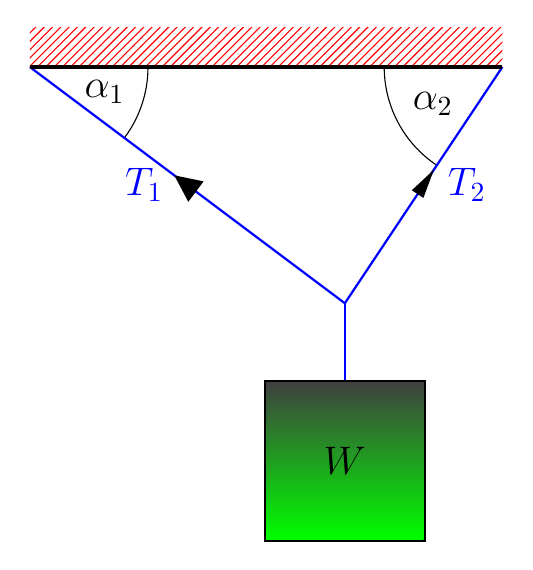
\begin{tikzpicture}
    %GRID
    %\draw[lightgray] (0,0) grid (6,6);
    %KOORDINANT 
    \coordinate (A) at (0,6);
    \coordinate (B) at (6,6);
    \coordinate (C) at (4,3);
    %ATAP
    \fill[pattern=north east lines, pattern color=red] (A) rectangle (6,6.5);
    %SUDUT
    \tkzMarkAngle[size=1.5](A,B,C);
    \tkzLabelAngle(A,B,C){\Large $\alpha_2$};
    
    \tkzMarkAngle[size=1.5](C,A,B);
    \tkzLabelAngle(C,A,B){\Large $\alpha_1$};
    %TALI
    \draw[thick, color=blue] (C) -- (B) node[currarrow, pos=0.5, scale=1, xscale=2, sloped, color=black]{} node [midway, right=5pt]{\Large $T_2$};
    \draw[thick, color=blue] (C) -- (A) node [currarrow, sloped, scale=2, xscale=-1, pos=0.5, color=black]{} node [midway, left=5pt]{\Large $T_1$};
    \draw[thick, color=blue] (C) -- (4,1);
    \draw[ultra thick] (A) -- (B);
    %KOTAK
    \draw[ultra thick] (3,0) rectangle (5,2);
    \shade[top color=darkgray, bottom color=green] (3,0) rectangle (5,2) node [midway]{\Large $W$};
    \end{tikzpicture}
\end{center}
    \begin{enumerate}
        \item $\frac{W}{5}$
        \item $\frac{W}{4}$
        \item $\frac{W}{3}$
        \item $\frac{W}{2}$
        \item $\frac{2W}{3}$
    \end{enumerate}
   
%19% 
\item Sebuah silinder pejal bermassa $M$ dan berjari-jari $R$ bergerak menggelinding murni pada suatu bidang miring dengan kemiringan $\alpha$ terhadap bidang horizontal. Momone inersia silinder pejal terhadap sumbunya adalah $\frac{1}{2}MR^2$. Percepatan silinder pejal menuruni bidang miring adalah\dots
    \begin{enumerate}
        \item $\frac{1}{2}g \sin{\alpha}$
        \item $\frac{2}{3}g \sin{\alpha}$
        \item $\frac{3}{4}g \sin{\alpha}$
        \item $g \sin{\alpha}$
        \item $\frac{3}{2}g \sin{\alpha}$
    \end{enumerate}
    
%20%
\item Balok bermassa $M = 3 \; kg$ yang terpasang pada tali bermassa $m = 1$ gram dan panjang $L = 1,5$ meter berada pada keadaan diam pada suatu bidaang miring licin dengan kemiringan $30^\circ$. Waktu yang diperlukan bagi gelombang transversal untuk bergerak dari satu ujung tali ke ujung tali yang lain adalah\dots
\begin{center}
    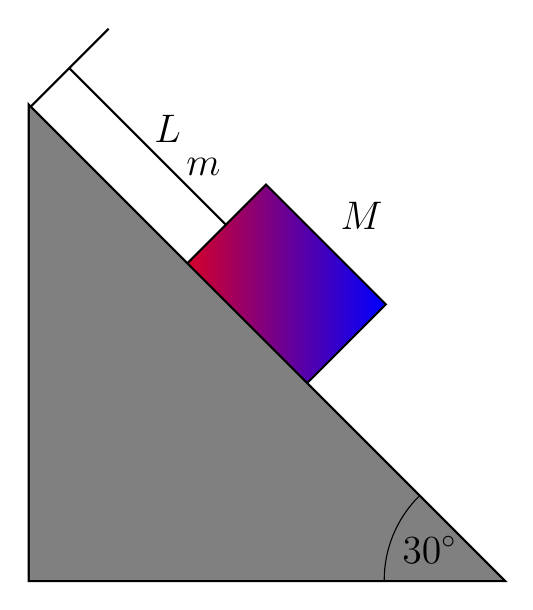
\begin{tikzpicture}
        %GRID
        %\draw[lightgray] (0,0) grid (7,7);
        %KOORDINAT
        \coordinate (A) at (0,0);
        \coordinate (B) at (6,0);
        \coordinate (C) at (0,6);
        %TALI % TEMBOK
        \draw[thick] (C) -- (1,7);
        \draw[thick] (0.5,6.5) -- (3,4) node[midway, above=5pt]{\Large $L$} node[midway, right=3pt]{\Large $m$};
        %KOTAK
        \draw[ultra thick] (3,5) -- node[midway, above right=2pt]{\Large $M$} (4.5,3.5) -- (3,2) -- (1.5,3.5) -- cycle;
        \shade[right color=blue, left color=red] (3,5) -- (4.5,3.5) -- (3,2) -- (1.5,3.5) -- cycle;
        %SEGITIGA
        \draw[ultra thick] (A) -- (B) -- (C) -- cycle;
        \fill[gray] (A) -- (B) -- (C) -- cycle;
        %SUDUT
        \tkzMarkAngle[size=1.5](C,B,A);
        \tkzLabelAngle(C,B,A){\Large $30^\circ$};
    \end{tikzpicture}
\end{center}
    \begin{enumerate}
        \item $0,01$ detik
        \item $0,02$ detik
        \item $0,05$ detik
        \item $0,1$ detik
        \item $0,2$ detik
    \end{enumerate}

%21%
\item Keika sebuah gulungan kawat pemanas diberi beda potensial $100 \; V$ ternyata dapat menaikkan suhu $1 \; kg$ air $10^\circ \; C$ dalam waktu $11$ sekon. Besar kenaikkan suhu $2 \; kg$ air yang dipanaskan dengan gulungan kawat tadi bila diberi beda potensial $200 \; V$ dalam $50$ sekon adalah\dots
    \begin{enumerate}
        \item $5^\circ \; C$
        \item $10^\circ \; C$
        \item $15^\circ \; C$
        \item $20^\circ \; C$
        \item $25^\circ \; C$
    \end{enumerate}
    
%22% 
\item Pada gas ideal yang mengalami ekspansi isobarik pada tekanan tetap $P$, suhu gas berubah dari $T_1$ ke $T_2$. Jika volume gas pada $T_1$ adalah $V_1$, besarnya usaha yang dilakukan pada ekspansi isobarik ini adalah\dots
    \begin{enumerate}
        \item $\frac{PV_1}{T_1}\left( T_2 - T_1 \right)$
        \item $\frac{PV_1}{T_1}T_2$
        \item $\frac{PV_1}{T_2}\left( T_2 - T_1 \right)$
        \item $\frac{PV_1}{T_2}T_1$
        \item $PV_1\frac{T_2-T_1}{T_2+T_1}$
    \end{enumerate}

%23%
\item Benda bersuhu $x^\circ \; C$ ketika diukur dengan menggunakan termometer Fahrenheit menunjukkan skala $2x^\circ \; F$. Nilai $x$ adalah\dots
    \begin{enumerate}
        \item $200$
        \item $180$
        \item $160$
        \item $140$
        \item $120$
    \end{enumerate}
    
%24%  
\item Empat muatan titik masing-masing $\left(+ \right)Q$, ditempatkan pada titik-titik sudut suatu bujur sangkar dengan panjang sisi-sisinya $l$. Besar gaya yang dialami oleh masing-masing muatan adalah\dots \\
\textbf{($k=$ tetapan Coulomb)}
	\begin{enumerate}
		\item $2 \frac{Q^2}{l^2}$
		\item $\sqrt{2} \frac{Q^2}{l^2}$
		\item $\left( \frac{1}{2} + \sqrt{2} \right) \frac{Q^2}{l^2}$
		\item $\frac{1}{2}\sqrt{2} \frac{Q^2}{l^2}$
		\item $\left( \sqrt{2} - \frac{1}{2} \right) \frac{Q^2}{l^2}$
	\end{enumerate}

%25%
\item Dua buah kapasitor identik yang mula-mula belum bermuatan akan dihubungkan dengan baterai. Bila hanya satu kapasitor yang dihubungkan dengan baterai $10 \; V$, energi yang tersimpan dalam kapasitor adalah $U$. Berapa energi yang tersimpan jika dua kapasitor tersebut dihubungkan secara seri dengan baterai?
   \begin{enumerate}
        \item $U^2$
        \item $2U$
        \item $U$
        \item $\frac{1}{2}U$
        \item $\frac{1}{2}U^2$
   \end{enumerate}
   
%26%
\item Tinjau suatu rangkaian listrik sebagaimana diberikan pada gambar. Jika nilai tiap hambatan adalah sama sebesar $R=1 \; \Omega$, hitunglah arus yang mengalir pada baterai.
\begin{center}
    \begin{tikzpicture}
        %GRID
        %\draw[lightgray] (0,0) grid (5,10);
        %KOORDINAT
        \coordinate (H) at (0,0);
        \coordinate (I) at (4,0);
        \coordinate[label=right:\Large $C$] (J) at (4,4);
        \coordinate[label=right:\Large $B$] (K) at (4,8);
        \coordinate (L) at (0,8);
        \coordinate[label=left:\Large $A$] (M) at (0,4);
        %NAMA POIN
        \tkzLabelAngle (J){$C$}
        %RANGKAIAN
        \draw[very thick] (K) to[resistor, a={\Large $R$}] (M);
        
        \draw[very thick] (J) to[resistor, a={\Large $R$}] (M);
        
        \draw[very thick] (I) to[battery1, a={\Large $E=12 \; V$}] (H) -- (M) to[resistor, a={\Large $R$}] (L) to[resistor, a={\Large $R$}] (K) to[resistor, a={\Large $R$}] (J) to[resistor, a={\Large $R$}] (I);      
    \end{tikzpicture}
\end{center}
    \begin{enumerate}
        \item $\frac{96}{17}$
        \item $\frac{96}{16}$
        \item $\frac{96}{15}$
        \item $\frac{96}{14}$
        \item $\frac{96}{13}$
    \end{enumerate}
  
%27%  
\item Ada 100 kawat panjang yang terletak sejajar satu sama lain dengan arah arus listrik yang sama. Besarnya arus setiap kawat adalah $I$. Jarak antar kawat adalah $d$. Besarnya gaya persatuan panjang pada kawat paling pinggir adalah $f_1$, sedangkan gaya persatuan panjang pada kawat kedua dari pinggir adalah $f_2$. Jika selisih kedua gaya persatuan panjang tersebut dituliskan sebagai $k \frac{\mu_0 I^2}{2\pi d}$, maka nilai $k$ adalah\dots
    \begin{enumerate}
        \item $\frac{100}{99}$
        \item $\frac{101}{100}$
        \item $1$
        \item $\frac{100}{101}$
        \item $\frac{99}{100}$
    \end{enumerate}

%28%  
\item Dua buah partikel bermassa dan bermuatan yang identik bergerak melingkar beraturan masing-masing pada dua buah siklotron dengan medan magnet masing-masing adalah $B_1$ dan $B_2$. Jari-jari lintasan partikel masing-masing adalah $R_1$ dan $R_2$. Perbandingan energi kinetik kedua partikel tersebut $\frac{Ek_1}{Ek_2}$ adalah\dots
    \begin{enumerate}
        \item $\frac{B_1R_1}{B_2R_2}$
        \item $\frac{B_1R_2}{B_2R_1}$
        \item $\frac{B^2_1R^2_1}{B^2_2R^2_2}$
        \item $\frac{B^2_1R^2_2}{B^2_2R^2_1}$
        \item $\frac{B_1R^2_1}{B_2R^2_2}$
    \end{enumerate}

%29%  
\item Sebuah partikel mengalami gerak harmonik sederhana dengan frekuensi $10 \; Hz$ dan amplitudo $13 \; cm$. Saat kecepatan partikel sama dengan $2,4\pi \; m/s$, simpangan partikel sama dengan\dots
    \begin{enumerate}
        \item $12 \; cm$
        \item $8 \; cm$
        \item $0 \; cm$
        \item $-5 \; cm$
        \item $-10 \; cm$
    \end{enumerate}

%30%
\item Benda bermassa $2 \; kg$ bergetar selaras sederhana. Ketika benda tersebut berada di titik setimbang kecepatannya $2 \; m/s$ dan ketika di simpangan $20 \; cm$ benda itu diam. Benda tersebut mengalami gaya yang dapat dinyatakan sebagai\dots
    \begin{enumerate}
        \item $F = -400 \; x$
        \item $F = -200 \; x$
        \item $F = -100 \; x$
        \item $F = -20 \; x$
        \item $F = -10 \; x$
    \end{enumerate}
 
%31%
\item Sebuah lensa bikoveks simetris berjari-jari $10 \; cm$ memiliki indeks bias $\frac{3}{2}$. Jarak fokus lensa tersebut jika berada di dalam air dengan indeks bias $\frac{4}{3}$ adalah\dots
    \begin{enumerate}
        \item $20 \; cm$
        \item $24 \; cm$
        \item $36 \; cm$
        \item $40 \; cm$
        \item $48 \; cm$
    \end{enumerate}

%32%
\item Benda hitam pada suhu $277^\circ \; C$ memancarkan radiasi dengan intensitas $5 \times 10^4 \; W/m^2$. Pada suhu $727^\circ \; C$ intensitas radiasi benda hitam tersebut dalam $10^4 \; W/m^2$ :
    \begin{enumerate}
        \item $20$
        \item $40$
        \item $80$
        \item $500$
        \item $800$
    \end{enumerate}

%33%
\item Setelah rentang waktu $t_1$ aktivitas suatu zat radioaktif berkurang dari $N_0$ ke $N_1$. Tetapan peluruhan zat radioaktif tersebut adalah\dots
    \begin{enumerate}
        \item $\frac{1}{t_1}\left( \ln N_1 - \ln N_0 \right)$
        \item $\frac{1}{t_1}\left( \ln N_1 + \ln N_0 \right)$
        \item $\frac{1}{t_1}\left( \ln N_0 - \ln N_1 \right)$
        \item $t_1 \left( \ln N_0 - \ln N_1 \right)$
        \item $t_1 \left( \ln N_1 + \ln N_0 \right)$
    \end{enumerate}

%34%
\item Bila $m$ adalah massa diam elektron dan $c$ adalah kecepatan cahaya maka besar usaha yang harus dilakukan pada sebuah elektron untuk mengubah kecepatan dari $0.6 \; c$ menjadi $0.8 \; c$ adalah\dots$mc^2$
    \begin{enumerate}
        \item $\frac{2}{9}$
        \item $\frac{3}{10}$
        \item $\frac{4}11}$
        \item $\frac{5}{12}$
        \item $\frac{6}{13}$
    \end{enumerate}

%35%
\item Sebuah pesawat bergerak terhadap bumi, dimana energi diam pesawat tersebut adalah empat kali energi kinetiknya. Pesawat tersebut melepaskan peluru dengan arah yang sama seperti arah gerak pesawat dimana menurut pesawat, energi diam peluru adalah $\frac{3}{2}$ kali energi kinetiknya. Menurut bumi, kecepatan peluru tersebut adalah\dots
    \begin{enumerate}
        \item $\frac{25}{28} \; c$
        \item $\frac{28}{30} \; c$
        \item $\frac{30}{32} \; c$
        \item $\frac{32}{35} \; c$
        \item $\frac{35}{37} \; c$
    \end{enumerate}

\end{enumerate}
\end{document}  
